\newpage
\section{Verification of Lossy Channel Systems}
\label{model}
The goal of this chapter is to formalize the use of \e{small models} for the verification of lossy channel systems, as is done in \cite{parosh}. The technique is based on the use of \e{abstract interpretation} techniques, first formalized by Cousot and Cousot\cite{cousot1977}. Abstract interpretation techniques are techniques for approximating programs. Using information about the control and data flow, i.e. the semantics of a system, an overapproximation of the possible configurations of a system can be created, which may result in an infinite set of configurations. In \cite{parosh} the authors show that such an infinite set of configurations can be safely bounded to a finite set of configurations, by finding a \e{cut-off} point for the maximum size of the evaluations.


\subsection{Views}
\label{subwords}
We define a \e{view} $v= \conf{s, \xi}$ to be a minimal representation of a set of configurations $C_v$, such that for any $c \in C_v$, $v \subword c$. Note that a view is itself a configuration, as they have the same representation, and we use the same terminology and notation for them, for example $size(v)$ to denote the size. The difference is that a configuration is a single entity, whereas the view is an abstract representation of a larger set of configurations.

\begin{exmp}
Let the view $v = \conf{(s_1, r_1), ab, cd}$, then the set $C_v$ is an infinite set, s.t. $\conf{(s_1, r_1), ab, cd} \in C_v$, $\conf{(s_1, r_1), abab, cdcd} \in C_v$ but $\conf{(s_1, r_1), ab, \epsilon} \notin C_v$
\end{exmp}

\subsection{Abstraction function}
\label{alphagamma}
For a given parameter $k \in \mathbb{N}$, we use $C$ and $V$ to denote sets of configurations and views respectively, and $C_k$ and $V_k$ to denote the set of all configurations and views respectively of size up to $k$.

The abstraction function $\alpha_k: C\rightarrow 2^{V_k}$ maps a configuration $c$ into a set $V'$ of views of size up to $k$, such that for each $v\in V'$, $v \subword c$ and $size(v) \leq k$.

\paragraph{Example.} Suppose \e{c} is a configuration $\conf{s, ab,de}$. The configuration is of size 2 and $\alpha_2(c)$ is the set


\begin{ttabulartwo}
$\conf{s,ab,de}$ &
$\conf{s,a,de}$ &
$\conf{s,b,de}$ &
$\conf{s,\epsilon,de}$ \\
$\conf{s,ab,d}$ & 
$\conf{s,a,d}$ &
$\conf{s,b,d}$ &
$\conf{s,\epsilon,d}$ \\
$\conf{s,ab,e}$ &
$\conf{s,a,e}$ &
$\conf{s,b,e}$ &
$\conf{s,\epsilon,e}$ \\
$\conf{s,ab, \epsilon}$ &
$\conf{s,a, \epsilon}$ &
$\conf{s,b, \epsilon}$ &
$\conf{s,\epsilon,\epsilon}$ \\
\end{ttabulartwo}


\subsection{Concretization function}
The concretization function $\gamma_k: 2^{V_k} \rightarrow 2^C$ returns, for a given set of views \e{V'}, the set of configurations that can be reconstructed from the views in $V'$, in other words, $\gamma_k(V') = \{c \in C$ | $\alpha_k(c) \subseteq V'$\}

In general $\gamma_k(V')$ is an infinite set of configurations. We define $\gamma_k^l(V')$ := $\gamma_k(V') \cap C_l$ for some $l\geq 0$. The intuitive meaning is that $\gamma_k^l(V')$ is the set of configurations of size at most $l$ for which all views of length at most $k$ are in $V'$.

\subsection{Post-Image}
For a configuration $c\in C$ of a lossy transition system $LTS = (C,\rightarrow)$, we define the \e{post-image} of \e{c} denoted $\rho(c)$ = \{$c'$ | $c \rightarrow c'$\}. Intuitively, the post-image of a configuration is the configuration obtained by firing the transitions of the transition system.

For a \e{set} of configurations $V'$ we define the post-image of the set $\rho(V')$ = \{$c' | c \rightarrow c', c \in V'$\}. This means that the post-image of a set $V'$ of configurations is the set $\rho(V')$ containing the post-images of each configurations $c\in V'$.

\subsection{Abstract Post-Image}
The \e{abstract post-image} of a set \e{V'} $\subseteq$ $C_k$ is defined as $Apost_k$(\e{V'}) = $\alpha_k(\rho(\gamma_k(V')))$. This means that the abstract post-image of a set $V'$ is the set obtained by applying $\gamma_k$, $\rho$ and $\alpha_k$ in order to the set $V'$. The procedure is illustrated in figure \ref{apost}.
\begin{figure}
\abstraction
\caption{The application order of the $\alpha$, $\rho$ and $\gamma$}
\label{apost}
\end{figure}

Note that since $V' \subseteq Apost_k(V')$, $Apost_k$ is a monotonic function, thus by the Knaster-Tarski theorem, the function $Apost_k$ has a fixpoint.
%\todo[inline]{Even the infinite powerset must reach a fixpoint, right?}

\subsection{Reachability Analysis}
\label{reachcompute}
Let LTS be a lossy transition system, with an initial configuration $c^0$. Then the set of reachable configurations $\mathcal{R}$ of LTS can be computed inductively as follows: $A_0 = \{c^0\}, A_{i+1}= A_i \cup \rho(A_i)$. The finite set of configurations $\mathcal{R}_k$ with size at most $k$ can be similarly computed; $A_0$ = $\{c^0\}$, $A_{i+1} = A_i \cup (\rho(A_i) \cap C_k)$.

\subsection{Small Models}
\label{proof}
Calculating the abstract post-image of a set of views $V' \subseteq V_k$ is essential for the verification procedure. As $\gamma_k(V')$ typically is infinite, this cannot be done straightforwardly. The main result of ~\cite{parosh} that it suffices to consider configurations of $\gamma_k(V')$ of sizes up to $k+1$ (i.e. $\gamma_k^{k+1}$), which is a finite set of configurations for which the abstract post-image can be computed. Formally, they show that

\begin{lemma}
\label{lemma1}
For any $k\in\mathbb{N}$, and $V'\subseteq V_k$, $\alpha_k(\rho(\gamma_k(V')))$ $\cup$ $V'$ = $\alpha_k(\rho(\gamma_k^{k+1}(V')))$ $\cup$ $V'$.
\end{lemma}
%\todo{Why is this correct? Shouldn't it be the fixpoint of the two that is equal?}

\begin{proof}
We want to show that the set $\gamma_k^{k+1}(V')$ of views of size at most $k+1$ is an abstract representation of the full set $\gamma_k(V')$. In order to do this, 
%we need to show that for any reachable configuration $c$ of larger size than $k+1$, all the views of $c$ of size at most $k$ are included in the set $\gamma_k(X)$ (i.e., the configuration $c$ is abstractly represented). More precisely, 
we want to show that for any configuration $c \in$ $\rho(\gamma_k(V'))$ of size $m > k + 1$ such that there is a transition  $c' \xrightarrow{r} c$, then for each view $v' \in$ $\alpha_k(c)$, the following holds: There is a configuration $d'$ $\in$ $\gamma_k^{k+1}(V')$ of size at most $k+1$ and transition $ d' \xrightarrow{r} d$ s.t. $v \in$ $\alpha_k(d)$.
\end{proof}

Note that by design (see section \ref{LTS}), transitions only change a single evaluation, therefore, although the set of evaluations may contain multiple evaluation, we direct our focus to a single evaluation in this section.

\paragraph{Transmissions}
\label{proofTransmission}
Consider a configuration $c' = \conf{s', x} \in \gamma_k(V')$ and a transition $r: c' \xrightarrow{ch!m} c = \conf{s,x \bullet m}$. Any view $v = \conf{s', y}$ of size at most $k$ of $c$ is on one of the following forms:

\begin{enumerate}
\item
$y \subword x$, $|y| \leq k$. In this case, the set $\gamma_k^{k+1}(V')$ includes all the configurations $d'$ = $\conf{s', y}$, as $d_E' \subword c_E'$. Then $d' \xrightarrow{ch!m} d$ yields $d = \conf{s, y\bullet m}$, for which $\conf{s, y} = v$ is a view.
\item
$y = z\bullet m$ with $z \subword x$, $|z| \leq (k-1)$. The set $\gamma_k^{k+1}(V')$ includes all the configurations $d'$ = $\conf{s', z}$, as $d_E' \leq c_E'$. Then $d' \xrightarrow{ch!m} d$ yields $d = \conf{s, z\bullet m}$ which is of size at most $k$, meaning it is also a view, $d$ = $v$.
\end{enumerate}


\paragraph{Actions}
Consider a configuration $c' = \conf{s', x} \in \gamma_k(V')$ and a transition $r: c' \xrightarrow{a} c = \conf{s, x}$. Since $r$ is an action, it can be fired regardless of the channel evaluation. Therefore, if $r$ can be fired from the configuration $c'$, it may also be fired from any view $v' = \conf{s', y}$ of size at most $k$ of $c'$, resulting in a view $v =  \conf{s, y}$.

Let $\{\conf{s', w_1}, \conf{s', w_2}, \ldots,  \conf{s', w_n}\}$ be the views of $c'$, then the transition $r$ can be fired from each of these, resulting in a set $\{\conf{s, w_1}, \conf{s, w_2},\ldots \conf{s, w_n}\}$, which is the complete set of views of size at most $k$ of $c$, showing that $c$ is abstractly represented in $\gamma_k(V')$.

\paragraph{Receptions and Message Loss}
Note that receptions transitions can be seen as a special case of a message loss, where messages are lost in FIFO order, i.e. a proof of lemma 1 for message loss directly applies to the reception transitions. Consider a configuration $c' = \conf{s', x} \in \gamma_k(V')$ and a transition $r: c' \xrightarrow{*} c = \conf{s', y}$. Since $y \subword x$, the set of views $V$ of $c$ is a subset of the set of views $V'$ of $c'$.

\subsection{Verification Algorithm}
\label{verificationalgorithm}
Suppose $Bad$ is a set of bad configurations, such that $|b| = 0$ for all $b \in Bad$. As a result of lemma \ref{lemma1}, if $\gamma_k^{k+1}(V_k) \cap Bad$ = $\emptyset$ for any \e{k} $\geq$ $1$, then $\gamma_l^{l+1}(V_k) \cap Bad$ = $\emptyset$ for any $l \geq k$. Given a set of bad configurations \e{Bad}, a set of initial configurations \e{I} and a set of transitions, verification of a system can be done with algorithm \ref{alg1}, which was first presented in \cite{parosh}.

\begin{algorithm}
\begin{algorithmic}[1]
  \caption{General Verification algorithm}
  \label{alg1}
    \State \hspace{8pt}\textbf{for} $k := 1$ \textbf{to} $\infty$

    \State \hspace{16pt}\textbf{if} $\mathcal{R}_k$ $\cap$ $Bad$ $\neq$ $\emptyset$ \textbf{then return} Unsafe

    \State \hspace{16pt}$V_k := \mu X.\alpha_k(I)$ $\cup$ $Apost_k(X)$

    \State \hspace{16pt}\textbf{if} {$\gamma_k(V_k)$ $\cap$ $Bad$ = $\emptyset$} \textbf{then return} Safe
\end{algorithmic}
\end{algorithm}

The algorithm begins by performing a reachability analysis, as explained in \ref{reachcompute} in order to compute $\mathcal{R}_k$ and check for bad configurations. For any buffer size \e{k}, if a bad configuration is found to be reachable in $\mathcal{R}_k$, the system is unsafe and the algorithm terminates. If no such bad state was found, the algorithm continues by computing a set of configurations $V'$, for which the set of concretizations $\gamma_k^{k+1}(V_k)$ is an \e{overapproximation} of reachable configurations of size $k$, reachable through configurations of size at most $k+1$ and checking for bad configurations. This is done by computing the fixpoint of $Apost_k$. If at this point no bad configuration has been found, the system can be said to be safe and the algorithm terminates. If on the other hand a bad state was found, the system is not necessarily unsafe, as $V_k$ is an overapproximation of the reachable states in $\mathcal{R}_k$. The process is then repeated with a buffer size of \e{k+1}. This process is abstractly described in the flowchart in figure \ref{flow}.

\begin{figure}
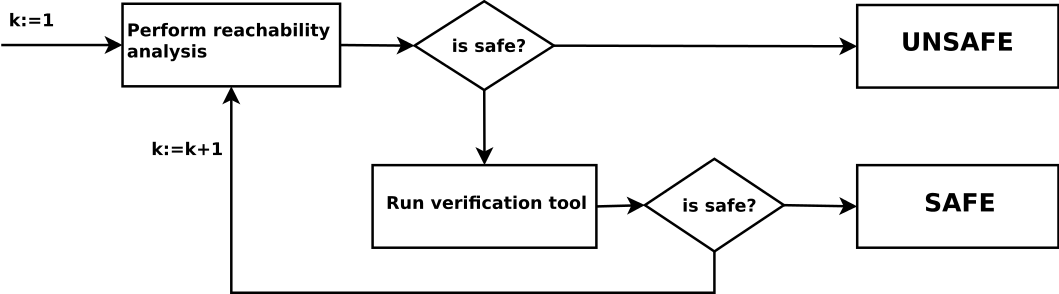
\includegraphics[width=400pt] {bilder/flowchart.png}
\caption{The general flow of the verifier.}
\label{flow}
\end{figure}
